% ----------------------------------------------------------
\chapter{Materiais e Métodos}\label{cap:metodos}
% ----------------------------------------------------------

Este capítulo descreve a bancada de aquisição, as calibrações, o processamento das imagens, a construção dos conjuntos de dados, o treinamento dos dois classificadores (a LUT de cor e a CNN de defeitos), a interface de operação e o protocolo de avaliação. Trata-se de uma pesquisa aplicada, de abordagem quantitativa e caráter experimental. A \autoref{fig:fluxo} resume o processamento de cada imagem: após o balanço de branco, os tomates são segmentados e, para cada um, são calculados o tamanho, a maturação e a probabilidade de defeito; a maturação e o defeito determinam o destino do fruto, e o tamanho é apenas medido e registrado.

\begin{figure}[htb]
	\caption{\label{fig:fluxo}Fluxo de processamento de uma imagem da bancada.}
	\centering
	\small
	\setlength{\fboxsep}{4pt}
	\fbox{Imagem da câmera} $\rightarrow$ \fbox{Balanço de branco} $\rightarrow$ \fbox{Segmentação (Otsu)} $\rightarrow$
	\fbox{\begin{tabular}{l}Tamanho e forma (escala por região)\\ Maturação (LUT de cor)\\ Defeito (CNN ResNet-18)\end{tabular}} $\rightarrow$ \fbox{Destino}
	\fonte{Elaborado pelo autor (2026).}
\end{figure}

O sistema foi implementado em Python, com a biblioteca OpenCV para o processamento de imagens e a inferência da CNN, a biblioteca scikit-learn para o \textit{k-means} e a MLP e o PyTorch para o treinamento da CNN. O código foi organizado em módulos pequenos e testáveis, com testes automatizados de unidade para a segmentação, a medição, a LUT, a inspeção e as métricas.

% ----------------------------------------------------------
\section{Bancada de Aquisição}
% ----------------------------------------------------------

A bancada consiste em uma caixa escura fechada, projetada para bloquear a luz ambiente, com a câmera fixa apontada para baixo a 303 mm do fundo (\autoref{fig:caixa}). Foi usada a câmera de um telefone celular, ligada ao computador pelo aplicativo DroidCam, com resolução de 1920 $\times$ 1080 pixels. O fundo é um tecido sintético preto e fosco, escolhido para contrastar com frutos de qualquer cor e para reduzir reflexos. Na imagem, apenas uma região de interesse retangular de 938 $\times$ 588 pixels (cerca de 188 $\times$ 118 mm) é processada; objetos que tocam a borda dessa região são descartados, pois parte deles não está visível.
% FIXME (autor): informar o modelo do celular e o custo aproximado dos componentes (celular, caixa, iluminação, computador), para sustentar o termo "baixo custo".
% FIXME (autor): descrever a iluminação usada (tipo de lâmpada/LED, posição, difusor) e se foco, exposição e balanço de branco da câmera foram travados no aplicativo.

\begin{figure}[htb]
	\caption{\label{fig:caixa}Caixa escura da bancada (modelo 3D).}
	\centering
	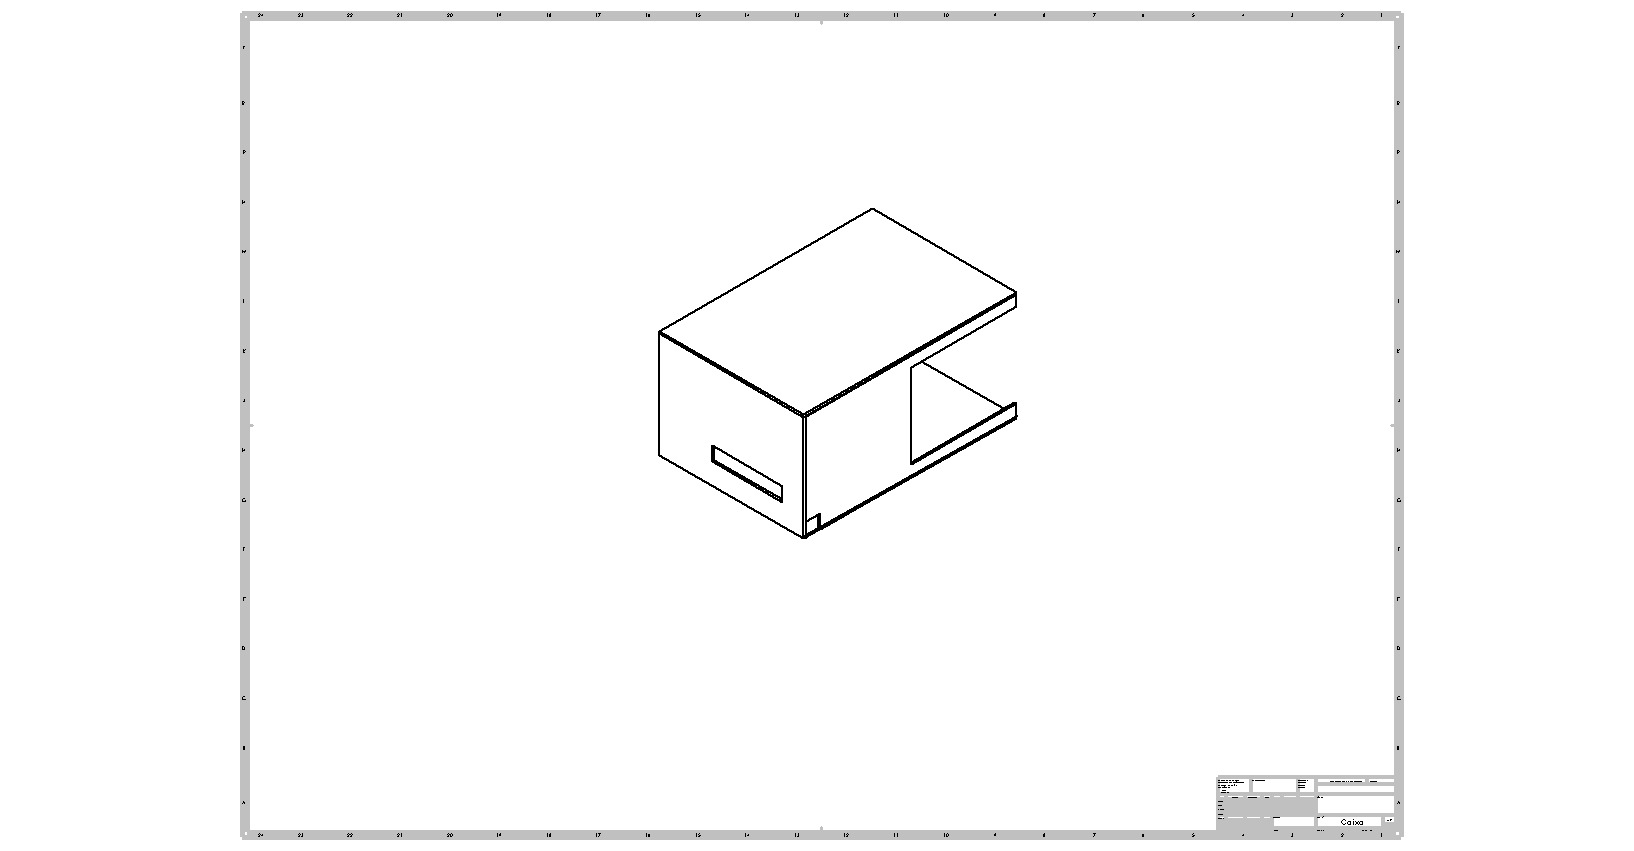
\includegraphics[width=0.85\textwidth]{images/caixa.jpg}
	\fonte{Elaborado pelo autor (2026).}
\end{figure}

% ----------------------------------------------------------
\section{Calibrações}
% ----------------------------------------------------------

\subsection{Balanço de branco}

Com uma folha branca na bancada, mede-se a média de cada canal na região de interesse e calcula-se um ganho por canal que leve essa média a um nível-alvo de 230, conforme o modelo diagonal de von Kries descrito no \autoref{cap:revisao}. Os ganhos obtidos foram 2,33 (R), 1,78 (G) e 1,48 (B): a luz da bancada era fria e a exposição, baixa, o que exigiu um ganho elevado no canal vermelho. O programa também mede a variação do branco ao longo da região, para detectar iluminação não uniforme; o canal vermelho variou 14,7\%, acima do limite de 8\% adotado como alerta, o que é discutido como limitação no \autoref{cap:resultados}. Todos os ganhos são aplicados a cada imagem antes de qualquer outro processamento, tanto no treinamento quanto na operação.

\subsection{Escala por região}

A escala foi calibrada com um tabuleiro de xadrez impresso com quadrados de 15 mm, colocado no plano do fundo. Os cantos internos foram detectados pelo método de \textcite{duda2018}, implementado no OpenCV. A região de interesse foi dividida em uma grade de 3 $\times$ 3 células e, em cada célula, a escala (mm/pixel) foi estimada como a média de 15 mm dividido pelo comprimento, em pixels, de cada segmento entre cantos vizinhos cujo ponto médio cai na célula. A \autoref{fig:escala} mostra o resultado: a escala variou de 0,1966 a 0,2038 mm/pixel, com média de 0,2008 mm/pixel, diminuindo de cima para baixo na imagem, padrão compatível com uma pequena inclinação da câmera em relação ao plano.

\begin{figure}[htb]
	\caption{\label{fig:escala}Calibração da escala por região com tabuleiro de 15 mm: escala (mm/pixel) e erro estimado em cada célula.}
	\centering
	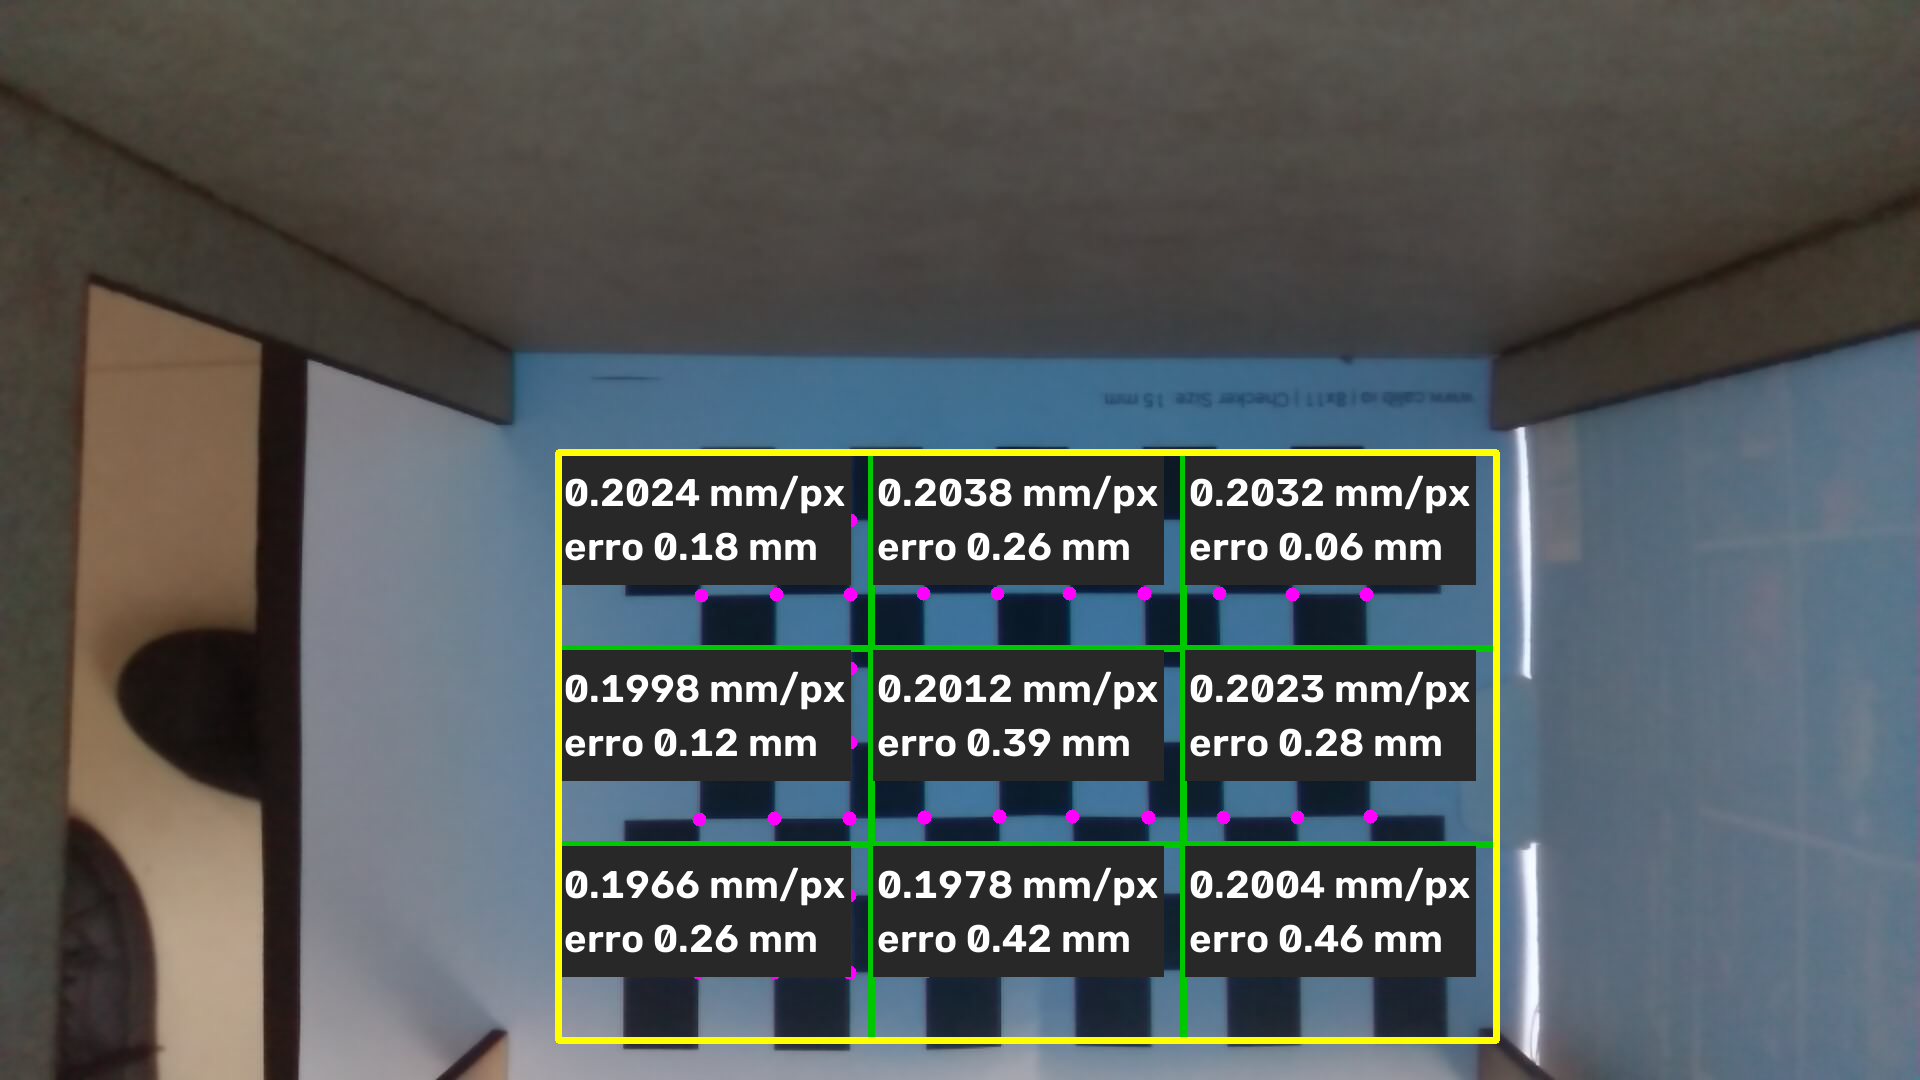
\includegraphics[width=0.9\textwidth]{images/bancada_escala.png}
	\fonte{Elaborado pelo autor (2026).}
\end{figure}

Para medir um objeto, cada um dos seus pixels é convertido em área (mm$^2$) com a escala da célula em que ele está, e o diâmetro equivalente é calculado a partir da área total. Assim, um objeto sobre a divisa entre células usa a escala de cada parte.

% ----------------------------------------------------------
\section{Segmentação e Medição}
% ----------------------------------------------------------

A segmentação segue o método descrito no \autoref{cap:revisao}. Na imagem com balanço de branco, calcula-se, para cada pixel, o maior valor entre os canais R, G e B, o que mantém contrastados contra o fundo preto tanto os frutos vermelhos quanto os verdes. Essa imagem é suavizada com filtro gaussiano de 5 $\times$ 5 pixels e limiarizada pelo método de Otsu. Em seguida, aplicam-se abertura (elemento estruturante elíptico de 5 pixels) e fechamento (9 pixels), e os contornos externos encontrados são preenchidos. Um objeto só é aceito se a diferença entre o seu brilho médio e o do fundo for de pelo menos 30 níveis; sem essa verificação, em uma imagem sem tomate o limiar de Otsu dividiria o próprio ruído do fundo em duas classes.

Para cada tomate segmentado, são calculados:
\begin{alineas}
	\item o diâmetro equivalente em milímetros, com a escala por região;
	\item o comprimento e a largura, dados pelos lados do menor retângulo girado que contém o contorno, multiplicados pela escala efetiva do fruto (raiz da razão entre a área em mm$^2$ e a área em pixels);
	\item a circularidade, $4\pi A/P^2$, em que $A$ é a área e $P$ o perímetro em pixels.
\end{alineas}

A medição foi validada com uma moeda de R\$ 1,00, de diâmetro nominal 27,00 mm, fotografada 64 vezes em todas as células da grade, com e sem a correção por região.

% ----------------------------------------------------------
\section{Conjuntos de Dados}
% ----------------------------------------------------------

Os tomates-cereja foram adquiridos em supermercado e fotografados na bancada com um programa de captura desenvolvido neste trabalho, que grava a foto e uma linha de rótulos em um arquivo CSV: número do tomate, defeitos presentes (rachado, podre ou mofado, dano mecânico e mancha) e estádio de maturação. Um tomate é considerado sadio quando não tem nenhum defeito marcado. O estádio de maturação é um campo opcional do programa; ele foi preenchido no conjunto de cor e no de teste, mas não nas sessões do conjunto de defeitos. Os rótulos foram atribuídos por inspeção visual do autor. Os tomates vieram de supermercado, e não diretamente de produtores, o que pode não representar a variedade de defeitos encontrada na origem. Foram formados três conjuntos, sempre com tomates distintos entre si:
% FIXME (autor): informar se algum defeito foi provocado (queda, pressão, imersão em água) ou se todos são naturais, e quantas compras/lotes foram usados.

\begin{alineas}
	\item \textbf{conjunto de cor}: 51 fotos (50 aproveitáveis) de 32 tomates com maturação informada (2 imaturos, 7 intermediários e 23 maduros), usado para gerar a LUT;
	\item \textbf{conjunto de defeitos}: 259 fotos aproveitáveis de 97 tomates, 49 sadios (140 fotos) e 48 com defeito (119 fotos), usado no treinamento e na validação cruzada da CNN. Das 266 fotos registradas na planilha de rótulos, 5 (de dois tomates) não tinham o arquivo de imagem correspondente e foram excluídas e 2 (de um mesmo tomate) foram descartadas porque o fruto não ficou inteiro dentro da região de interesse. Cerca de 40\% dos tomates foram fotografados em várias posições, girando o fruto entre as fotos (até 11 fotos por tomate); os demais têm uma foto. Entre os tomates com defeito, 25 têm mancha, 19 dano mecânico, 12 podridão ou mofo e 3 rachadura; 9 têm mais de um defeito;
	\item \textbf{conjunto de teste}: 22 tomates, uma foto cada, que não foram usados no treinamento de nenhum dos modelos, fotografados em 27/11/2026 logo após os últimos tomates do conjunto de defeitos: 9 sadios e 13 com defeito; 17 maduros, 4 intermediários e 1 imaturo.
\end{alineas}

Na primeira sessão de captura (tomates 1 a 29), todos os tomates sadios foram fotografados antes dos defeituosos. Como a ordem de captura pode se confundir com a classe (por exemplo, pelo aquecimento da câmera ou por pequenas mudanças de posição e de iluminação), as sessões seguintes e o conjunto de teste intercalaram, ao menos parcialmente, tomates sadios e defeituosos. A primeira sessão, porém, reúne 28 dos 97 tomates e 176 das 259 fotos do conjunto de defeitos, pois nela cada tomate foi fotografado várias vezes; o efeito dessa sessão é analisado no \autoref{cap:resultados}.

% ----------------------------------------------------------
\section{Classificação da Maturação por LUT}
% ----------------------------------------------------------

A LUT foi gerada em quatro etapas, conforme os fundamentos do \autoref{cap:revisao}:

\begin{alineas}
	\item \textbf{amostragem}: em cada foto do conjunto de cor, o tomate é segmentado e são sorteados até 4.000 pixels do seu interior (descartando uma faixa de 4 pixels junto à borda, onde a cor se mistura com o fundo) e 1.500 pixels do fundo;
	\item \textbf{agrupamento}: os pixels de tomate de todas as fotos, convertidos para L*a*b*, são agrupados em 8 grupos pelo \textit{k-means} com inicialização \textit{k-means++}. Um painel com a cor média e exemplos de cada grupo (\autoref{fig:grupos}) foi usado para dar nome a cada grupo entre verde, amarelado, rosado, vermelho e cálice;
	\item \textbf{treinamento da MLP}: uma MLP com duas camadas ocultas de 32 neurônios recebe as coordenadas L*a*b* normalizadas do pixel e prevê sua classe (as cores nomeadas mais o fundo). Para evitar que as classes mais frequentes dominem, cada classe contribui com até 20.000 pixels. Os pixels de cerca de 20\% dos tomates de cada maturação com pelo menos três tomates foram reservados para validação da MLP (sorteio por tomate); como o agrupamento usou todas as fotos, essa validação não é independente dos rótulos;
	\item \textbf{geração da tabela}: a MLP é avaliada uma única vez para as $256^3$ cores possíveis, e o resultado é gravado em uma tabela de 16,7 milhões de posições (cerca de 16 MB).
\end{alineas}

\begin{figure}[htb]
	\caption{\label{fig:grupos}Os oito grupos de cor do \textit{k-means}: cor média, fração dos pixels e exemplo de pixels de cada grupo.}
	\centering
	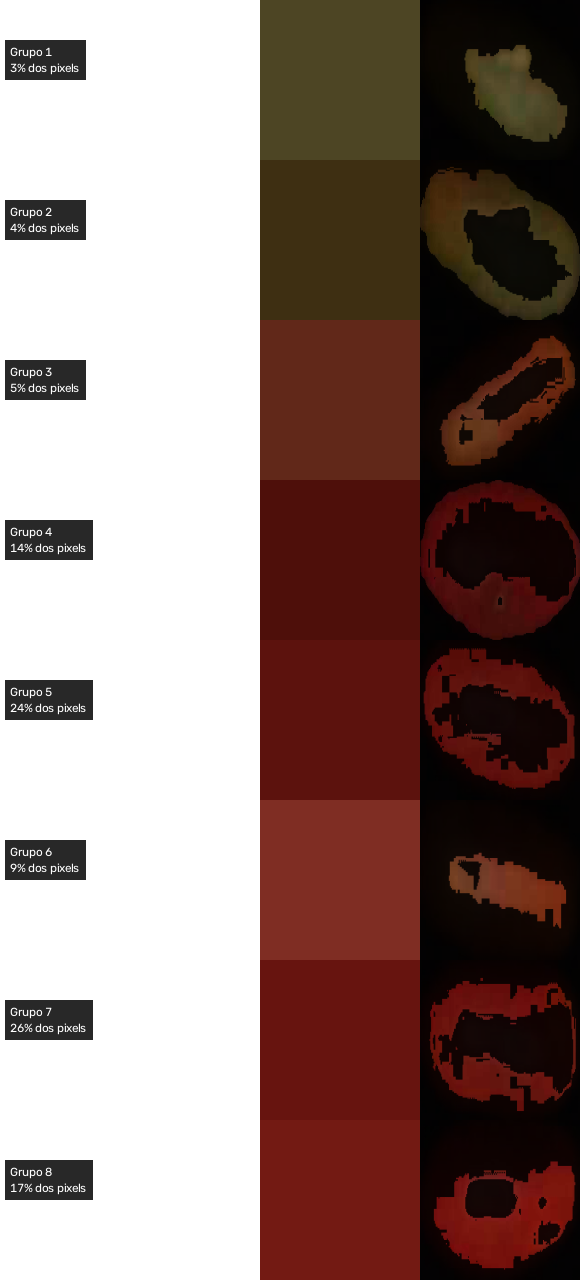
\includegraphics[height=0.55\textheight]{images/grupos_cor.png}
	\fonte{Elaborado pelo autor (2026).}
\end{figure}

Os grupos foram nomeados como verde (grupos 1 e 2), amarelado (3), rosado (6) e vermelho (4, 5, 7 e 8). Nenhum grupo correspondeu ao cálice, porque a segmentação e a amostragem do interior do fruto raramente o incluem.

Na operação, cada pixel do tomate é classificado por consulta à tabela, e a maturação é decidida pela proporção das cores, em uma adaptação dos estádios do USDA \cite{usda1991}:
\begin{alineas}
	\item \textbf{imaturo}: menos de 10\% da superfície colorida (amarelada, rosada ou vermelha), o que corresponde aos estádios verde e início de cor;
	\item \textbf{maduro}: mais de 60\% da superfície vermelha, correspondendo aos estádios vermelho claro e vermelho;
	\item \textbf{intermediário}: os demais casos (estádios virando e rosado).
\end{alineas}
Para o maduro, conta-se apenas o vermelho, e não qualquer cor, porque no padrão do USDA o amarelado caracteriza o início da mudança de cor; com a contagem de qualquer cor, um fruto inteiramente alaranjado seria classificado como maduro.

% ----------------------------------------------------------
\section{Detecção de Defeitos por CNN}
% ----------------------------------------------------------

\subsection{Entrada e arquitetura}

A entrada da CNN é um recorte quadrado em torno do tomate segmentado, com margem de 15\% do seu maior lado, redimensionado para 224 $\times$ 224 pixels, na imagem com balanço de branco. O fundo do recorte não é mascarado, pois a borda do fruto, onde costumam estar rachaduras e danos, poderia ser cortada por uma máscara imperfeita. A rede é uma ResNet-18 \cite{he2016} com os pesos pré-treinados no ImageNet \cite{deng2009}, cuja camada final foi substituída por uma camada totalmente conectada de duas saídas (sadio e com defeito). A normalização da entrada pela média e pelo desvio padrão do ImageNet foi incorporada ao próprio modelo, para que o programa de operação não precise reproduzi-la.

\subsection{Treinamento}

Toda a rede foi ajustada (\textit{fine-tuning}) com o otimizador AdamW \cite{loshchilov2019}, taxa de aprendizado de $10^{-4}$, penalização dos pesos de $10^{-4}$ e lotes de 16 imagens, minimizando a entropia cruzada ponderada pelo inverso da frequência de cada classe \cite{he2009}. O aumento de dados aplicou, a cada época, rotação aleatória de até 180$^\circ$, espelhamentos horizontal e vertical, recorte aleatório de 80\% a 100\% da área e pequenas variações de brilho, contraste e saturação (até 15\%, 15\% e 10\%). A matiz não foi alterada, para preservar a cor do fruto.

\subsection{Validação cruzada e modelo final}

O desempenho esperado em tomates novos foi estimado por validação cruzada em 5 partes, com divisão \emph{por tomate} e estratificada por classe (\textit{StratifiedGroupKFold}): todas as fotos de um tomate ficam na mesma parte, evitando o vazamento descrito por \textcite{kapoor2023}. Em cada parte, uma rede nova foi treinada por até 30 épocas, e a época com a maior acurácia balanceada na validação (com desempate pela menor perda) foi registrada. Como essa escolha usa os próprios dados de validação, a estimativa resultante é otimista \cite{cawley2010}, razão pela qual o desempenho final é medido no conjunto de teste. As métricas da validação cruzada são calculadas por foto; como um tomate pode ter até 11 fotos, os tomates muito fotografados pesam mais nessas médias.

O modelo final foi treinado com todos os tomates do conjunto de defeitos pelo número de épocas igual à mediana das melhores épocas das 5 partes. Separar tomates apenas para escolher a época retiraria exemplos de defeito, que são escassos. O modelo foi exportado no formato ONNX, com a função \textit{softmax} na saída, e é executado na operação pelo módulo de redes neurais do OpenCV, sem necessidade do PyTorch ou de placa de vídeo. Após a exportação, conferiu-se que as probabilidades calculadas pelo OpenCV coincidem com as do PyTorch em todas as imagens de treino (diferença máxima tolerada de 0,02). Um tomate é classificado como defeituoso quando a probabilidade de defeito é de pelo menos 0,5.

O treinamento foi executado em um computador com placa de vídeo NVIDIA GeForce RTX 3050.

% ----------------------------------------------------------
\section{Interface de Operação}
% ----------------------------------------------------------

A interface homem-máquina (IHM) foi desenvolvida com a biblioteca Tkinter. Ela mostra o vídeo da câmera restrito à região de interesse e, ao comando do operador (botão ou barra de espaço) ou em modo contínuo, inspeciona a imagem: cada tomate é contornado na cor do seu destino e numerado, e um cartão lateral apresenta, para cada fruto, o destino, a maturação com as porcentagens de superfície colorida e vermelha, a probabilidade de defeito, o diâmetro, o comprimento, a largura e a circularidade. Contadores mostram quantos frutos foram enviados a cada destino, e cada inspeção é registrada em um arquivo CSV diário.

O destino é decidido em duas etapas: um tomate com defeito vai para o descarte, qualquer que seja a sua cor; os demais são separados pela maturação (imaturo, intermediário ou maduro). Internamente, a inspeção completa de uma imagem é oferecida à interface por uma única classe (padrão de projeto \textit{Facade}), que encadeia balanço de branco, segmentação, medição, LUT e CNN; com isso, a mesma rotina é usada pela IHM e pela avaliação no conjunto de teste.

% ----------------------------------------------------------
\section{Protocolo de Avaliação}
% ----------------------------------------------------------

O conjunto de teste foi processado uma única vez, depois de concluídos a LUT e o modelo final da CNN, pela mesma rotina de inspeção da IHM, sem nenhum ajuste posterior de limiares ou modelos; a versão preliminar da CNN, treinada com 28 tomates, nunca foi aplicada a ele. Em cada foto, se mais de um objeto fosse segmentado, o maior seria tomado como o tomate. Foram calculados:

\begin{alineas}
	\item para a CNN, tomando ``com defeito'' como classe positiva: acurácia, sensibilidade, especificidade, acurácia balanceada, precisão e F1, além da matriz de confusão;
	\item para a LUT: a acurácia da maturação nas três classes e a matriz de confusão, em todos os tomates, com ou sem defeito;
	\item para o sistema completo: a acurácia do destino final, sendo esperado o descarte para os tomates com defeito e a classe de maturação rotulada para os sadios;
	\item o tempo de processamento por imagem, desde o balanço de branco até a decisão do destino.
\end{alineas}

A unidade de análise é o tomate. Para as proporções (acurácia, sensibilidade e especificidade), foram calculados intervalos de confiança de 95\% pelo método de \textcite{wilson1927}. Os critérios de aceitação definidos no início do projeto foram: segmentação correta em pelo menos 95\% das imagens; erro de até 0,5 mm na calibração da escala, medido pelo resíduo das distâncias entre cantos do próprio tabuleiro; erro médio absoluto de até 1 mm no diâmetro; acurácia de pelo menos 90\% na maturação; F1 de pelo menos 0,85 na classe ``com defeito''; e tempo de processamento de até 200 ms por tomate.
